\documentclass[12pt]{article}
\usepackage{amsmath}
\usepackage{mathtools}
\usepackage{tikz}

\begin{document}

\begin{center}
\large\bf University of Waterloo\\
CS~466 --- Advanced Algorithm\\
Spring 2013\\
Problem Set 4\\
Siwei Yang - 20258568\\
\end{center}
\bigskip

\begin{enumerate}

\item{} [6 marks: Splay Trees]
One feature of splaying versus the simple move to root heuristic is that in performing a splay operation (i.e. performing the appropriate splay operations to move a node to the root), no node has its depth increased by more than 2. Prove this.

Let's observe what happens when a splay operation fires off where x is the splay node, p and g are x's parent and grandparent.

\begin{center}
Zig:
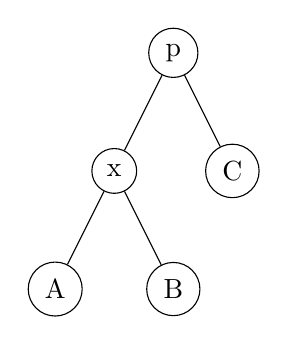
\begin{tikzpicture}
\node[circle,draw](z){p}
  child{
node[circle,draw]{x} child{node[circle,draw] {A}} child{node[circle,draw] {B}}
  }
  child{
node[circle,draw]{C}
  };
\end{tikzpicture}
becomes
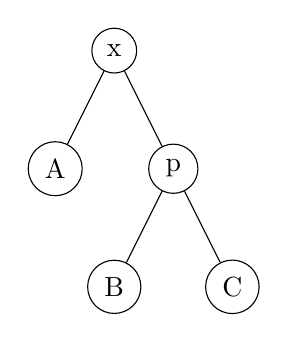
\begin{tikzpicture}
\node[circle,draw](z){x}
  child{
node[circle,draw]{A}
  }
  child{
node[circle,draw]{p} child{node[circle,draw] {B}} child{node[circle,draw] {C}}
  };
\end{tikzpicture}
\end{center}

\begin{center}
Zig-zig:
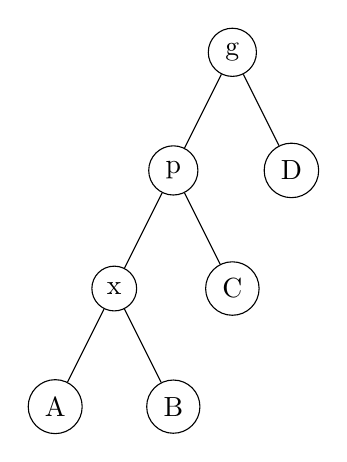
\begin{tikzpicture}
\node[circle,draw](z){g}
  child{
node[circle,draw]{p}
  child{
node[circle,draw] {x} child{node[circle,draw] {A}} child{node[circle,draw] {B}}
  }
  child{node[circle,draw] {C}}
  }
  child{
node[circle,draw]{D}
  };
\end{tikzpicture}
becomes
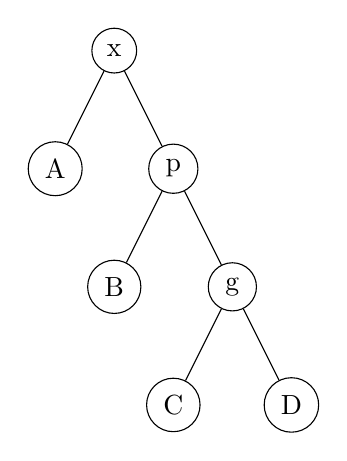
\begin{tikzpicture}
\node[circle,draw](z){x}
  child{
node[circle,draw]{A}
  }
  child{
node[circle,draw]{p}
  child{node[circle,draw] {B}}
  child{
node[circle,draw] {g} child{node[circle,draw] {C}} child{node[circle,draw] {D}}
  }
  };
\end{tikzpicture}
\end{center}

\begin{center}
Zig-zag:
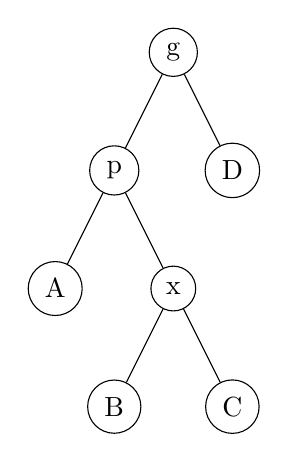
\begin{tikzpicture}
\node[circle,draw](z){g}
  child{
node[circle,draw]{p}
  child{node[circle,draw] {A}}
  child{
node[circle,draw] {x} child{node[circle,draw] {B}} child{node[circle,draw] {C}}
  }
  }
  child{
node[circle,draw]{D}
  };
\end{tikzpicture}
becomes
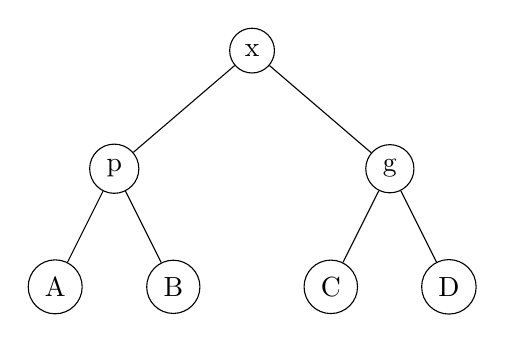
\begin{tikzpicture}
\node[circle,draw](z){x}
  child [xshift=-1cm]{
node[circle,draw]{p}
  child{node[circle,draw] {A}}
  child{node[circle,draw] {B}}
  }
  child [xshift=1cm]{
node[circle,draw]{g}
  child{node[circle,draw] {C}}
  child{node[circle,draw] {D}}
  };
\end{tikzpicture}
\end{center}

There are three other cases symmetrical to what listed above, but we will omit them for the sake of simplicity.

Through observation, we find for each splay step,
\begin{itemize}
\item all nodes affected becomes x's descendents
\item the nodes started as x's descendents will not increase their depth
\item the nodes becomes x's descendents will increase their depth at most by 2
\end{itemize}

And we know any node can become x's descendents at most once, and their depth won't increase after that. Thus, \textbf{during a full splay operation, no node has its depth increase by more than 2}.

\medskip

\item{} [6 marks: Close to 2-SAT]
Suppose you have a Boolean formula in CNF (conjunctive normal form) with n variables and also n clauses. However $\lg{n}$ clauses have three literals (variables or their negations) and the remaining ones have just two. Sketch an efficient algorithm to determine whether the formula is satisfiable.

The algorithm to solve the formula is to divide the problem into 3-SAT and 2-SAT problems. Then solve the 2 problems individually.

Let the original problem be F. The sub-problem only has 3 literals clauses is $F_{3-SAT}$. The sub-problem only has 2 literals clauses is $F_{2-SAT}$.
\begin{equation}
F = F_{3-SAT} \land F_{2-SAT}
\end{equation}

First tackle $F_{3-SAT}$ by enumerating all possible variable assignments of the variables in the formula. Consider the number of variables need to be covered:
\begin{equation}
| v(F_{3-SAT}) | \leq 3 * \lg{n}
\end{equation}

Thus, the size of the enumeration:
\begin{equation}
2^{| v(F_{3-SAT}) |} \leq n^{3}
\end{equation}

For each enumeration, it's a linear time operation to check if the assignment is valid. In case of a valid assignment, substitute the assignment into $F_{2-SAT}$ to arrive at $F_{2-SAT}'$. Use the linear algorithm taught in class to determine if $F_{2-SAT}'$ is satisfable. If $F_{2-SAT}'$ is satisfable, then $F$ is satisfable. Otherwise, move on to the next assignment for $F_{3-SAT}$. Unless at least one assignment creates a satisfable $F_{2-SAT}'$, the original problem $F$ is not satisfable. \textbf{The algorithm is a composite of three linear time operation, thus the algorithm is still linear time}.


\end{enumerate}

\end{document}

